\section{Ricerca della soglia di percolazione}
Per analizzare il comportamento della probabilità di percolazione $P_{perc}$ in funzione della probabilità di occupazione dei siti $p_{col}$, è stata condotta una serie di simulazioni su reticoli quadrati di diverse dimensioni ($L = 100$, $300$ e $1000$). L’intervallo di $p_{col}$ considerato va da $0.55$ a $0.65$, con incrementi di $0.01$, in modo da esplorare con buona risoluzione la zona critica.
\\\\
\noindent
Per ogni coppia di valori $(L, p_{col})$, l’esperimento è stato ripetuto $50$ volte, così da permettere una stima della probabilità di percolazione e del relativo errore. Ogni simulazione consiste nella generazione di un reticolo in cui ogni sito viene occupato con probabilità $p_{col}$. Una volta creato il reticolo, i cluster connessi di siti occupati sono stati individuati tramite l'algoritmo hk76. Successivamente, è stato verificato se esiste almeno un cluster che attraversa il reticolo da sinistra a destra (percolazione orizzontale) o dall’alto in basso (percolazione verticale).
\\\\
\noindent
Un confronto tra i risultati ottenuti nelle due direzioni ha permesso di confermare che, come previsto, tenendo conto dei relativi errori, la probabilità di percolazione orizzontale è la stessa di quella verticale.
\\\\
\textbf{Probabilità media di percolazione LR}
\\\\
\noindent
\begin{tabular}{|c|*{11}{c|}}
	\hline
	\textbf{}&\textbf{0.55} &	\textbf{0.56}& \textbf{0.57} &	\textbf{0.58}	& \textbf{0.59}& 	\textbf{0.60}&	\textbf{0.61}&\textbf{	0.62}&	\textbf{0.63}& \textbf{0.64} &\textbf{0.65}	\\
	\hline
	
	\textbf{100} &0.02 &	0.06& 0.06 &	0.18	& 0.38& 	0.60&	0.90&	0.94&	1.00 &	1.00 &	1.00\\
	\hline

	\textbf{300} & 0.00	& 0.00	& 0.00&	0.00&	0.30 & 0.82 &	0.98&	1.00&1.00&1.00&1.00\\
	\hline
	\textbf{1000}& 0.00&	0.00	&0.00	&0.00	&0.16&	0.98&	1.00&	1.00 & 1.00 & 1.00 & 1.00\\
	\hline
\end{tabular}
\vspace{15px}

\noindent
\textbf{Probabilità media di percolazione TB}

\vspace{15px}
\noindent
\begin{tabular}{|c|*{11}{c|}}
	\hline
	\textbf{}&\textbf{0.55} &	\textbf{0.56}& \textbf{0.57} &	\textbf{0.58}	& \textbf{0.59}& 	\textbf{0.60}&	\textbf{0.61}&\textbf{	0.62}&	\textbf{0.63}& \textbf{0.64} &\textbf{0.65}	\\
	\hline
	
	\textbf{100} &0.00 &	0.06 & 0.10	& 0.18	&0.48&	0.70&	0.82& 0.90&	1.00&	1.00&	1.00\\
	\hline
	\textbf{300}& 0.00	&0.00	&0.00	&0.02&	0.36&	0.86&	0.98&	1.00&	1.00	&1.00&	1.00 \\
	\hline
	\textbf{1000}&0.00	&0.00	&0.00	&0.00	&0.18&	1.00	&1.00	&1.00	&1.00&	1.00&	1.00\\
	\hline
\end{tabular}
\vspace{15px}

\noindent
\textbf{Errore nel calcolo di LR}

\vspace{15px}
\noindent
\begin{tabular}{|c|*{11}{c|}}
	\hline
	\textbf{} & \textbf{0.55} & \textbf{0.56} & \textbf{0.57} & \textbf{0.58} & \textbf{0.59} & \textbf{0.60} & \textbf{0.61} & \textbf{0.62} & \textbf{0.63} & \textbf{0.64} & \textbf{0.65} \\
	\hline
	\textbf{100}  & 0.02 & 0.03 & 0.03 & 0.05 & 0.07 & 0.07 & 0.04 & 0.03 & 0.00 & 0.00 & 0.00 \\
	\hline
	\textbf{300}  & 0.00 & 0.00 & 0.00 & 0.00 & 0.07 & 0.05 & 0.02 & 0.00 & 0.00 & 0.00 & 0.00 \\
	\hline
	\textbf{1000} & 0.00 & 0.00 & 0.00 & 0.00 & 0.05 & 0.02 & 0.00 & 0.00 & 0.00 & 0.00 & 0.00 \\
	\hline
\end{tabular}
\vspace{15px}

\noindent
\textbf{Errore nel calcolo di TB}

\vspace{15px}
\noindent
\begin{tabular}{|c|*{11}{c|}}
	\hline
	\textbf{} & \textbf{0.55} & \textbf{0.56} & \textbf{0.57} & \textbf{0.58} & \textbf{0.59} & \textbf{0.60} & \textbf{0.61} & \textbf{0.62} & \textbf{0.63} & \textbf{0.64} & \textbf{0.65} \\
	\hline
	\textbf{100}  & 0.00 & 0.03 & 0.04 & 0.05 & 0.07 & 0.07 & 0.05 & 0.04 & 0.00 & 0.00 & 0.00 \\
	\hline
	\textbf{300}  & 0.00 & 0.00 & 0.00 & 0.02 & 0.07 & 0.05 & 0.02 & 0.00 & 0.00 & 0.00 & 0.00 \\
	\hline
	\textbf{1000} & 0.00 & 0.00 & 0.00 & 0.00 & 0.05 & 0.00 & 0.00 & 0.00 & 0.00 & 0.00 & 0.00 \\
	\hline
\end{tabular}

\vspace{15px}
\noindent
Per ogni dimensione del reticolo $L$ è stata stimata la soglia di percolazione $p_c$ come il valore della probabilità di colorazione $p_{col}$ per cui la probabilità di percolazione $P_{perc}$ raggiunge il valore $0.5$.
\\\\
\noindent
Poiché i dati ottenuti tramite simulazione possono contenere duplicati (ad esempio valori estremi come $0.00$ e $1.00$), sono stati innanzitutto rimossi i punti ripetuti nei valori di $P_{perc}$.

\begin{figure}[H]
	\centering
	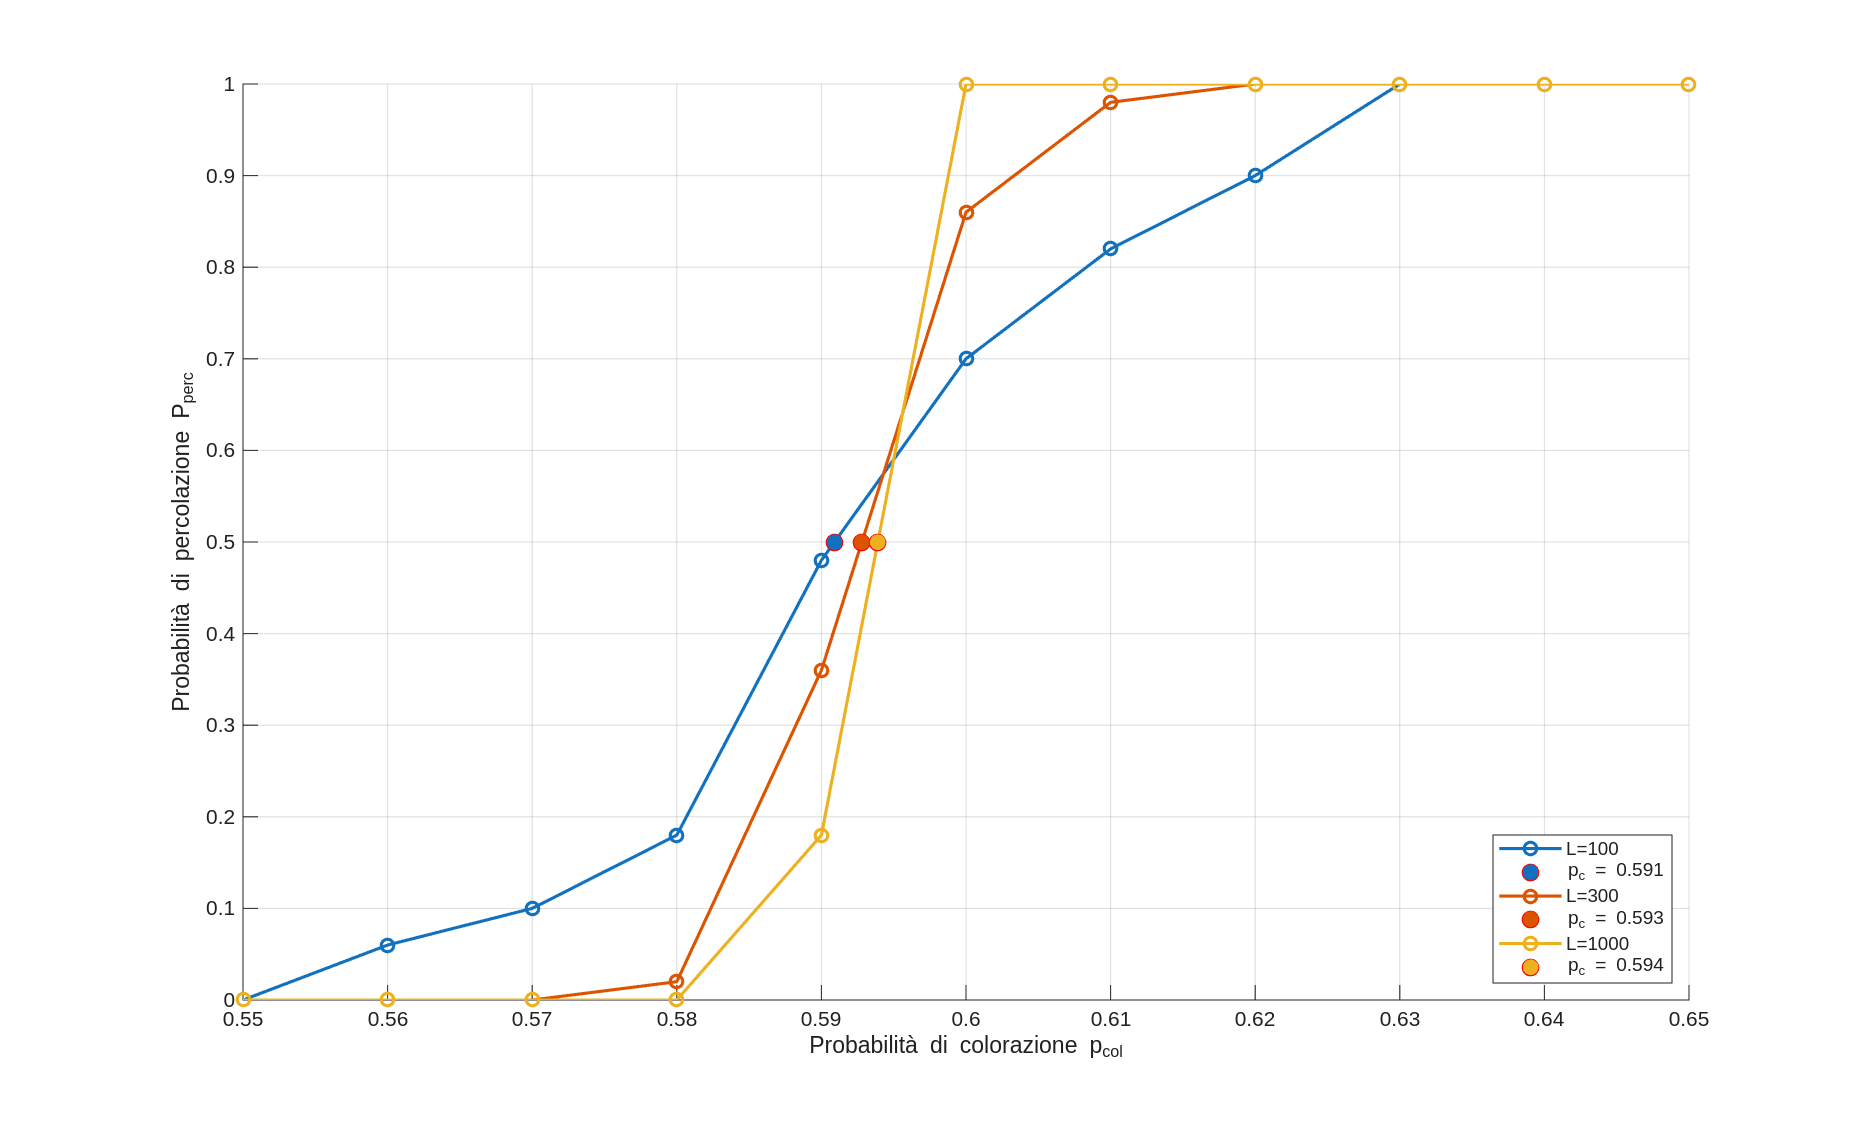
\includegraphics[width=\linewidth]{images/percolation_threshold.png}
	\caption{Andamento della probabilità di percolazione al variare di $p_{col}$.}
	\label{fig:perc_thr}
\end{figure}

\noindent
Successivamente, è stata utilizzata un’interpolazione lineare tra i punti ottenuti per stimare il valore di $p_{col}$ tale che $P_{perc} = 0.5$. Per ciascuna taglia del reticolo, il valore stimato di $p_c$ è stato evidenziato nel grafico in Figura~\ref{fig:perc_thr} come punto pieno sovrapposto alla curva $P_{perc}(p_{col})$. La procedura è stata ripetuta per tutte le dimensioni considerate, in modo da ottenere una stima della soglia di percolazione in funzione di $L$.
\\\\
\noindent
Questo approccio consente anche di osservare l’avvicinamento di $p_c(L)$ al valore critico nel limite termodinamico. In particolare, sulla base dei risultati ottenuti, questo valore asintotico è stimato attorno a $p_c \sim 0.59$.

